%%%%%%%%%%%%%%%%%%%%%%%%%%%%%%%%%%%%%%%%%%%%%%%
%%% Template for lab reports used at STIMA
%%%%%%%%%%%%%%%%%%%%%%%%%%%%%%%%%%%%%%%%%%%%%%%

%%%%%%%%%%%%%%%%%%%%%%%%%%%%%% Sets the document class for the document
% Openany is added to remove the book style of starting every new chapter on an odd page (not needed for reports)
\documentclass[10pt,english, openany]{book}

%%%%%%%%%%%%%%%%%%%%%%%%%%%%%% Loading packages that alter the style
\usepackage[]{graphicx}
% \documentclass[11pt, a4paper]{article}
\usepackage{graphicx}
\usepackage{amsmath}
\usepackage{listings}
\usepackage[]{color}
\usepackage{alltt}
\usepackage{amsmath, amssymb}
\usepackage[T1]{fontenc}
\usepackage[utf8]{inputenc}
\usepackage{lipsum}
\setcounter{secnumdepth}{3}
\setcounter{tocdepth}{3}
\setlength{\parskip}{\smallskipamount}
\setlength{\parindent}{0pt}

% Set page margins
\usepackage[top=100pt,bottom=100pt,left=68pt,right=66pt]{geometry}

% Package used for placeholder text
\usepackage{lipsum}

% Prevents LaTeX from filling out a page to the bottom
\raggedbottom

% Adding both languages
\usepackage[english]{babel}

% All page numbers positioned at the bottom of the page
\usepackage{fancyhdr}
\fancyhf{} % clear all header and footers
\fancyfoot[C]{\thepage}
\renewcommand{\headrulewidth}{0pt} % remove the header rule
\pagestyle{fancy}

% Changes the style of chapter headings
\usepackage{titlesec}
\titleformat{\chapter}
   {\normalfont\LARGE\bfseries}{\thechapter.}{1em}{}
% Change distance between chapter header and text
\titlespacing{\chapter}{0pt}{50pt}{2\baselineskip}

% Adds table captions above the table per default
\usepackage{float}
\floatstyle{plaintop}
\restylefloat{table}

% Adds space between caption and table
\usepackage[tableposition=top]{caption}

% Adds hyperlinks to references and ToC
\usepackage{hyperref}
\hypersetup{hidelinks,linkcolor = black} % Changes the link color to black and hides the hideous red border that usually is created

% If multiple images are to be added, a folder (path) with all the images can be added here 
\graphicspath{ {Figures/} }

% Separates the first part of the report/thesis in Roman numerals
\frontmatter


%%%%%%%%%%%%%%%%%%%%%%%%%%%%%% Starts the document
\begin{document}

%%% Selects the language to be used for the first couple of pages
\selectlanguage{english}

%%%%% Adds the title page
\begin{titlepage}
	\clearpage\thispagestyle{empty}
	\centering
	\vspace{1cm}

	% Titles
	% Information about the University
	{\Large Indian Institute of Technology, Madras \\ 
		Department of Electrical Engineering \\
		Applied Programming Lab \par}
		\vspace{3cm}
	{\LARGE \textbf{Lab Report}} \\
    \LARGE \textbf{Assignment 3} \\
	%\vspace{1cm}
	{\Huge \textbf{Fitting Data to Models} \par}
	\vspace{3cm}
	{\large \textbf{Nithin Uppalapati} \\ 
     \large \textbf{EE18B035} \\% \\ specifies a new line
	\vspace{2cm}
    
    \centering 
\includegraphics[scale=0.2]{IITm.pdf}
%     
    \vspace{1.5cm}
		
	% Set the date
	{\normalsize 11-02-2020 \par}
	
	\pagebreak

\end{titlepage}

% Adds a table of contents
\tableofcontents{}

%%%%%%%%%%%%%%%%%%%%%%%%%%%%%%%%%%%%%%%%%%%%%%%%%%%%%%%%%%%%%%%%%%%%%%%%%%%%%%%%%%%%%%%%%%%%
%%%%%%%%%%%%%%%%%%%%%%%%%%%%%%%%%%%%%%%%%%%%%%%%%%%%%%%%%%%%%%%%%%%%%%%%%%%%%%%%%%%%%%%%%%%%
%%%%% Text body starts here!\\
\mainmatter

\chapter{Abstract}\label{chapt:sum}
	\vspace{0.5cm}
	\large \textbf{Aim} : \par The aim of this project is to accurately fit the given data (measured data) to some specified functions. Specifically, in this assignment, we are fitting the data to a Bessel function of order 2 and a first order polynomial, both of them as a functions of time(\textit{t})\par
    \vspace{1cm}
   
    \large \textbf{Implementation} :  \par 
So, the method of prediction is as follows,
We proceed empirically, by assuming a set of valid range coefficients for the function and calculate the output of this ‘trial function’, and then we calculate the error of this ‘trial function’ with the actual output, by mean squared error method. Thus, we can predict the coefficients, by minimising the error.\par
\begingroup
\let\clearpage\relax
\chapter{Introduction}
Assignment 3 is based on
\begin{itemize}
\item Analysing the data to extract information by plotting graphs
\item Study the effect of noise on the fitting process using scipy, pylab libraries in python.
\item Plotting graphs using the pylab library
\end{itemize}

\endgroup
\chapter{Theory}
\vspace{0.5cm}
This assignment, is provided with a program named - "\textit{generatedata.py}" which creates the data to be fitted to the desired function, by adding a noise to the output of the actual function in the given range of time samples.\par
\vspace{0.2cm}

\vspace{1cm}
\section{Generating the Data}

\subsection{Generation of Noise}
We are producing the data from the given model, and adding a \textit{randomly generated} noise to it.
 The program ensures that the standard deviation of the noise is in the range of (0.001~0.1) and the standard deviation is chosen randomly and then is added to the actual data for the given range of time samples... 
 \par
 \subsection{Data File}
 The generated data should be collected and parsed from the file named "\textit{fitting.dat}", for collection of the "measured" data (data with noise) and the time samples. The data file consists of 10 columns. The first column is time, while the remaining columns are data. The data corresponds to the function : $f(t) = 1.05J(2, t) - 0.105t + n(t)$\par
 Where J(2, t) is Bessel function of order 2, imported from scipy.special library.\par
 The data can be collected from \textit{fitting.dat} in this way, as shown in the segment below:
 \begin{verbatim}
 f=open("fitting.dat")
dat=f.readlines()
N=len(dat)							# N=101, in the fit.data
k=len(dat[0].strip().split(' '))	#A=1.05
data=array([zeros(k)]*N)			#B=-0.105

for i in range(0,N):
	dat[i]=dat[i].strip()
	dat[i]=dat[i].split(' ')
	for j in range(0,k):
		data[i][j]=float(dat[i][j])
t=data[:,0]
y=g(t,A,B)

y_data=array([zeros(N)]*(k-1))
stdev=array(zeros(k-1))
for i in range(0,k-1):
	y_data[i]=data[:,i+1]
	stdev[i]=std(g(t,A,B)-y_data[i])
 \end{verbatim}
 where 
 \begin{verbatim}
 t=data[:,0]  ###corresponds to the first column in the data-array
 \end{verbatim}
\section{Analysing the Generated Data}
So, once the data and the time samples are collected, we store them in arrays of suitable sizes.\par
\begin{equation}
t=\begin{bmatrix} 
	t_0\\
    t_1\\
    t_2\\
    \vdots\\
    t_{100} \end{bmatrix}
    \end{equation}
    and the measured data(remaining columns other than the first one) matrix in the form:
   \begin{equation}
       y\_data=\begin{bmatrix} 
      	y_{0,1}&y_{0,2}&\cdots&y_{0,9}\\
   		y_{0,2}&y_{02}&\cdots&y_{0,9}\\
    	\vdots&\vdots &\ddots&\vdots\\
    	y_{100,n} &y_{100,2}&\cdots&y_{100,9}\end{bmatrix}
   \end{equation}   
   
 Now, create a matrix, with each column being a functional values (to the given time samples) to which the data to be fitted.\par
 \begin{equation}
F = 
 \begin{bmatrix}
 J(2, t) & t\\
 \end{bmatrix}
 \end{equation}
And also let us create the column matrix of the actual coefficients,
\begin{equation}
Coeff\_exact= 
 \begin{bmatrix}
 A&B\\
 \end{bmatrix}
 \end{equation}
 Where $A=1.05$ and $B=-0.105$ defined above
So, now we multiply this \textbf{functional values matrix} with a \textbf{guess matrix} of coefficients (where the coefficients are varied in the vicinity of the actual coefficients) and then the output of this multiplication is the predicted data, which should be compared with the measured data, and the error should be stored into an array.\par
And the guess coefficients matrix is generated by using:

\begin{verbatim}
A_guess=linspace(0,2,21)
B_guess=linspace(-0.2,0,21)
\end{verbatim}

\section{Minimising the Error}
 {\subsection{Mean Squared Error Method}} 
If a vector of n predictions generated from a sample of n data points on all variables, and Y is the vector of observed values of the variable being predicted, with $\hat Y_i$ being the predicted values (e.g. as from a least-squares fit), then the within-sample MSE of the predictor is computed as\par

$$ MSE = \frac{1}{n}\sum_{i=1}^{n} (Y_{i}-\hat{Y_{i}})^2$$

\subsection{Least Squares Method}
The method of least squares is a standard approach in regression analysis to approximate the solution of overdetermined systems (sets of equations in which there are more equations than unknowns) by minimizing the sum of the squares of the residuals made in the results of every single equation.
The most important application is in data fitting. The best fit in the least-squares sense minimizes the sum of squared residuals (a residual being: the difference between an observed value, and the fitted value provided by a model).\par
So, as the coefficients are varied to minimize the error, we differentiate the error wrt. each coefficient and equate it to zero, in order to obtain the vector of optimal coefficients ($p_i 's$).\par
And in python, in scipy.linalg library, there is a dedicated function, named $lstsq()$ [leastsqares], which accepts the arguments as : $lstsq(F,x)$

\section{Measure of Deviation from the Actual Data:}
\subsection{Standard Deviation of Noise in the Data}
\subsubsection{Actual Data with the noise added}
{\centering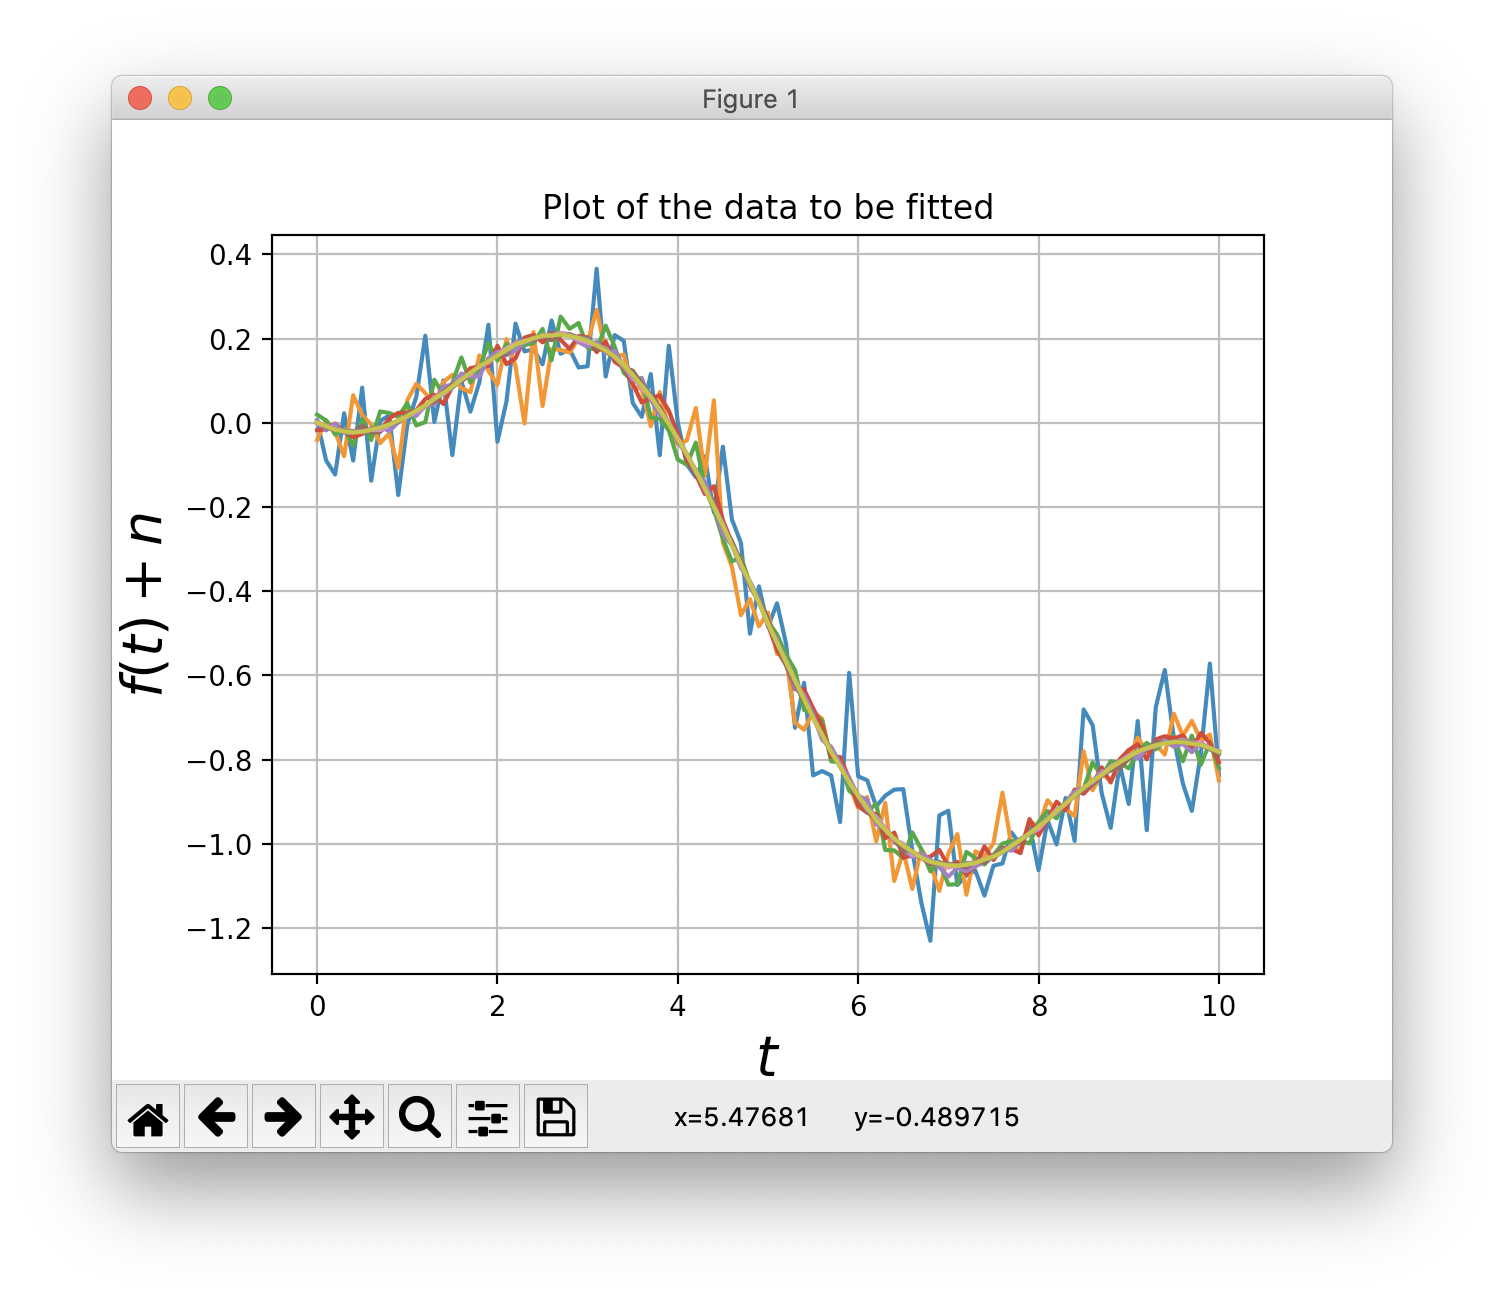
\includegraphics[scale=0.4]{scr5.png}}
The Standard deviation of the noise present in the data can be extacted by the inbuilt function, 
\begin{verbatim}
std(y\_data - g(t,A,B))
\end{verbatim}
and the standard deviation of the noise in each column is updated as follows:
\begin{verbatim}
for i in range(0,k-1):
	y_data[i]=data[:,i+1]
	stdev[i]=std(g(t,A,B)-y_data[i])
\end{verbatim}
%%%%%%%%%%%%%%%%%%%%%%
\subsection{Plotting Errorbars along with the Exact Function}
%%%%%%%%%%%%%%%%%%
\begin{verbatim}
errorbar(t[::5],y_data[i][::5],label="Errorbars",yerr=stdev[0],fmt="ro")
plot(t,y,label= "Exact function")
xlabel('noise standard deviation  ''$\longrightarrow$',size=15)
ylabel('A and B error  ''$\longrightarrow$',size=15)
\end{verbatim}
\subsubsection{Error Bar of Noisy Bessel Function relative to exact Bessel Function}
{\centering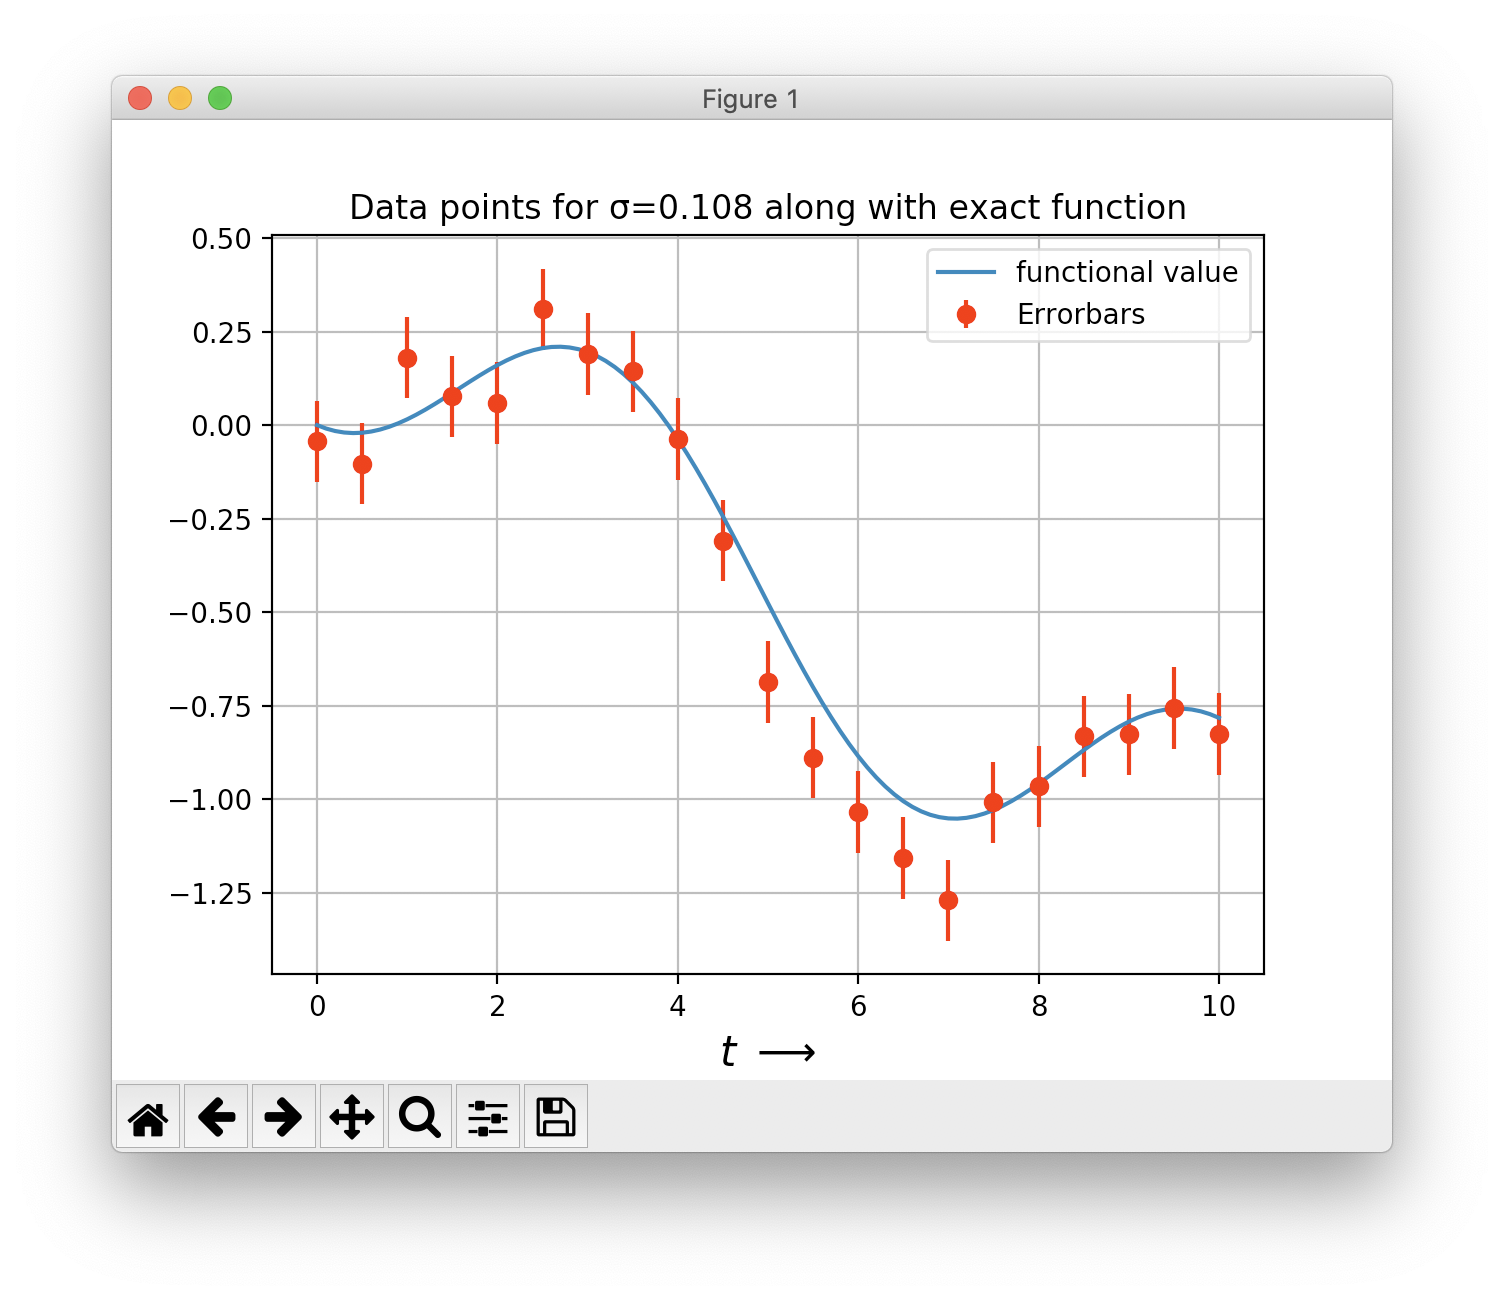
\includegraphics[scale=0.4]{scr4.png}}


\subsection{Plotting Errorbars in Variation of Error of Coefficients with noise}
\begin{verbatim}
errorbar(stdev,abs(A-predict_coeff[0]),yerr=std(A-predict_coeff[0]))
loglog(stdev,abs(A-predict_coeff[0]))
errorbar(stdev,abs(B-predict_coeff[1]),yerr=std(B-predict_coeff[1]))
loglog(stdev,abs(B-predict_coeff[1]))
xlabel('$\u03C3_n$' '  ' '$\longrightarrow$',size=15)
ylabel('A and B error  ''$\longrightarrow$',size=15)
title(r'Variation of error with noise__log plot')
\end{verbatim}

\subsubsection{Variation of \textbf{$A_{err}$} and \textbf{$B_{err}$} with $\sigma_{n}$ [Linear plot]}
{\centering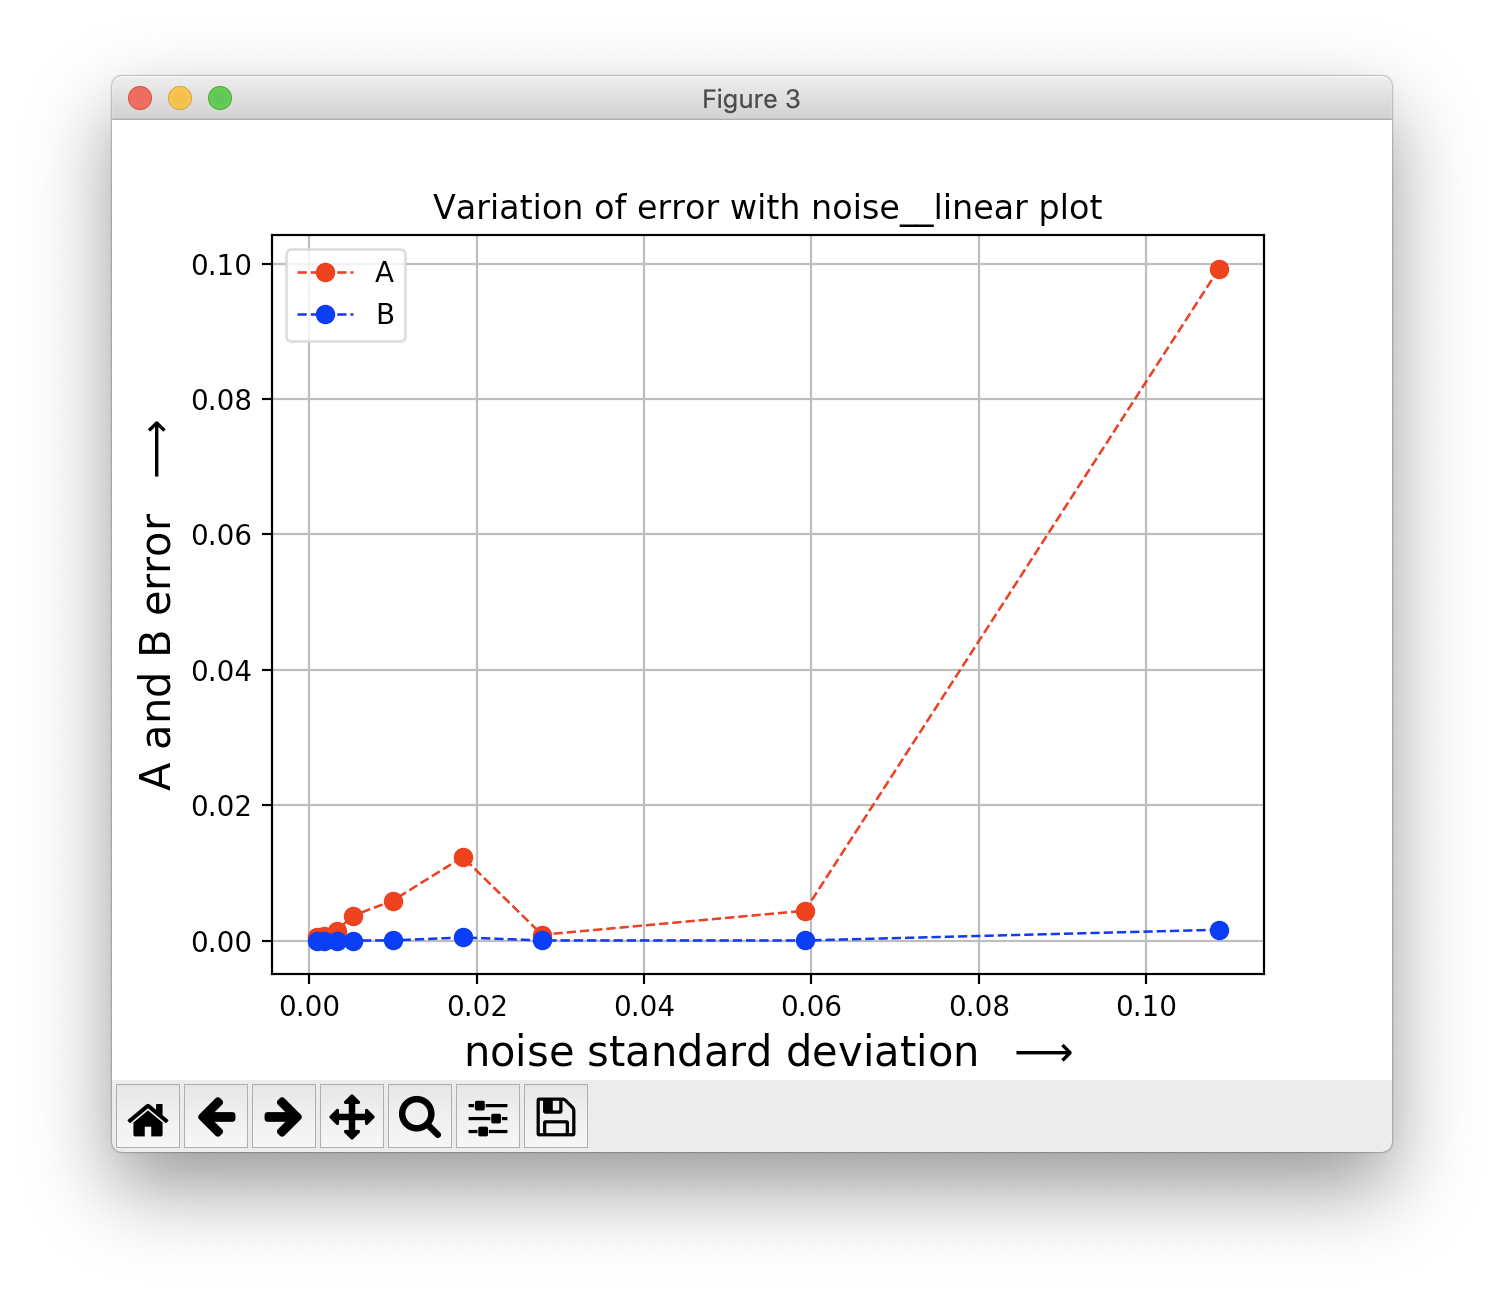
\includegraphics[scale=0.4]{scr2.png}}
\subsubsection{Variation of $A_{err}$ and $B_{err}$ with $\sigma_{n}$ [loglog plot]}
{\centering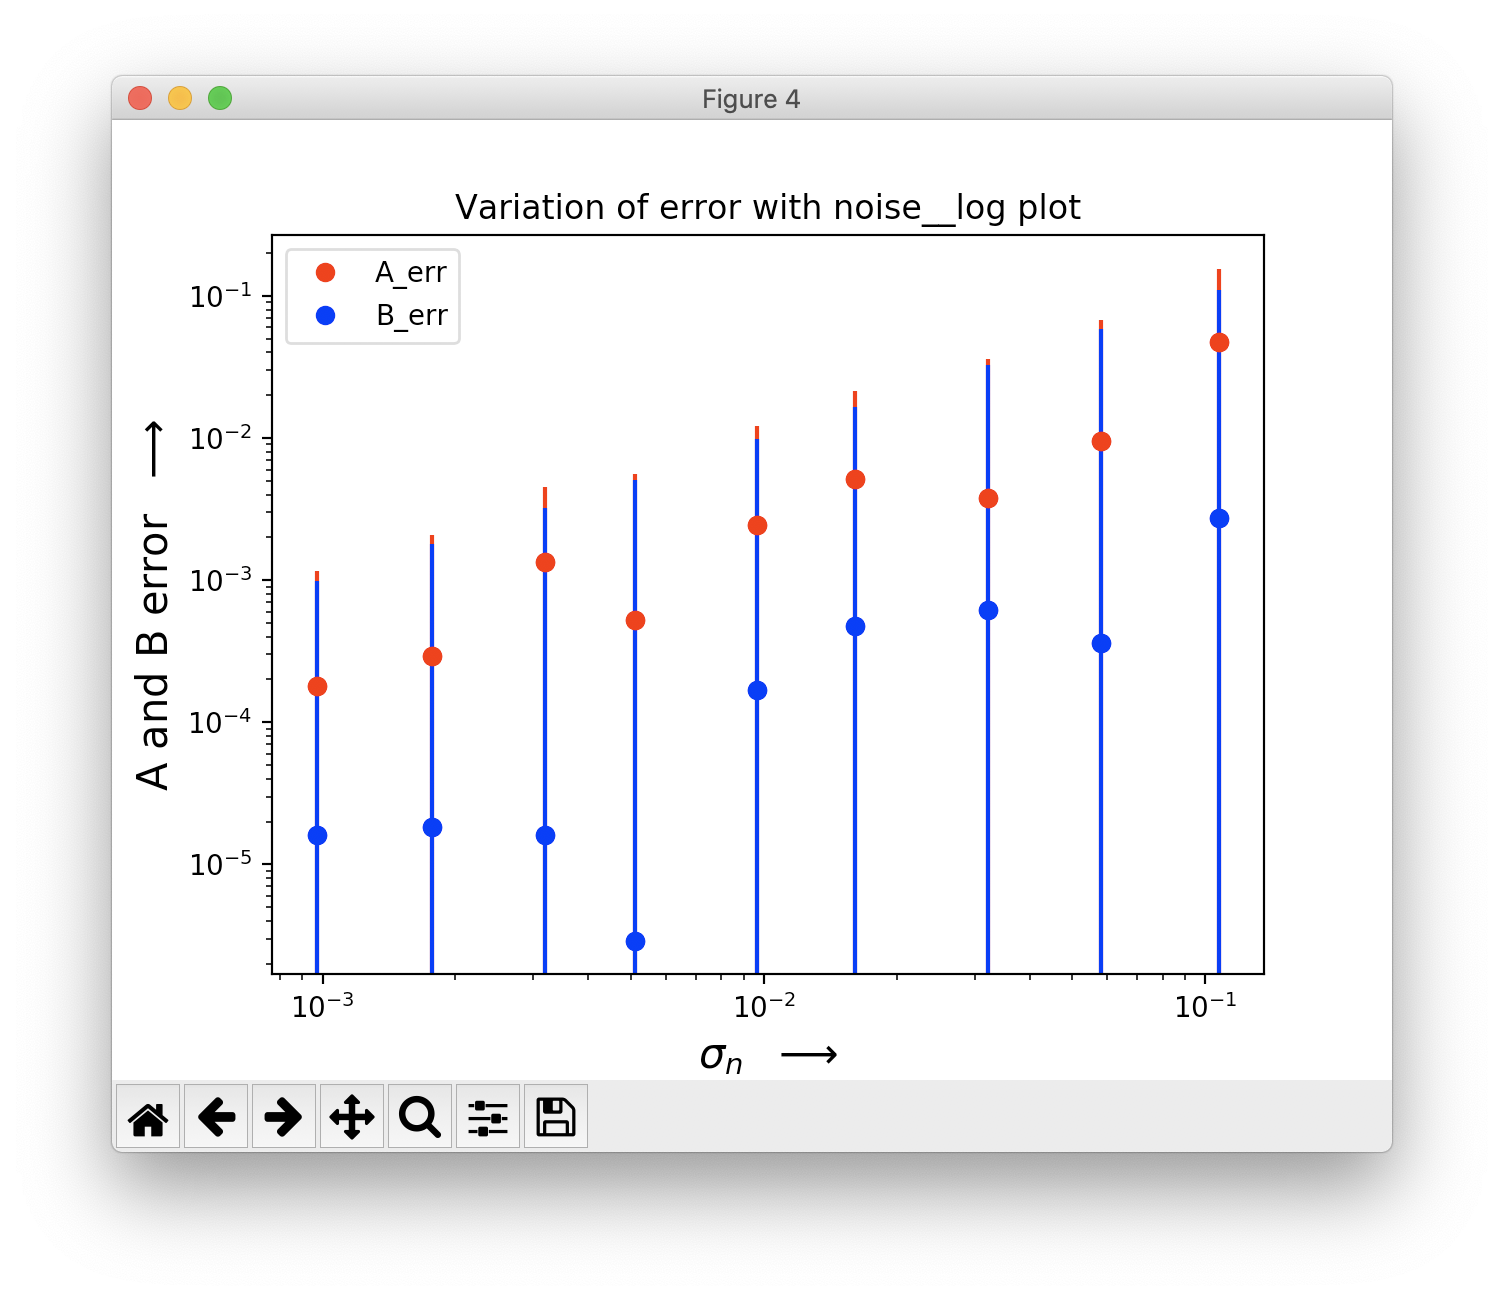
\includegraphics[scale=0.4]{scr1.png}}
\subsection{Calculating the Mean Squared Error}
\begin{verbatim}
A_guess=linspace(0,2,21)
B_guess=linspace(-0.2,0,21)
appx_err_val=array([zeros(21)]*21)

for i in range(0,21):
	for j in range(0,21):
		appx_err_val[i][j] = (square( y_data[0]-g(t,A_guess[i],B_guess[j]) )).mean()
\end{verbatim}

\subsubsection{Contour Plot of Noisy Bessel Function with varying A and B}
{\centering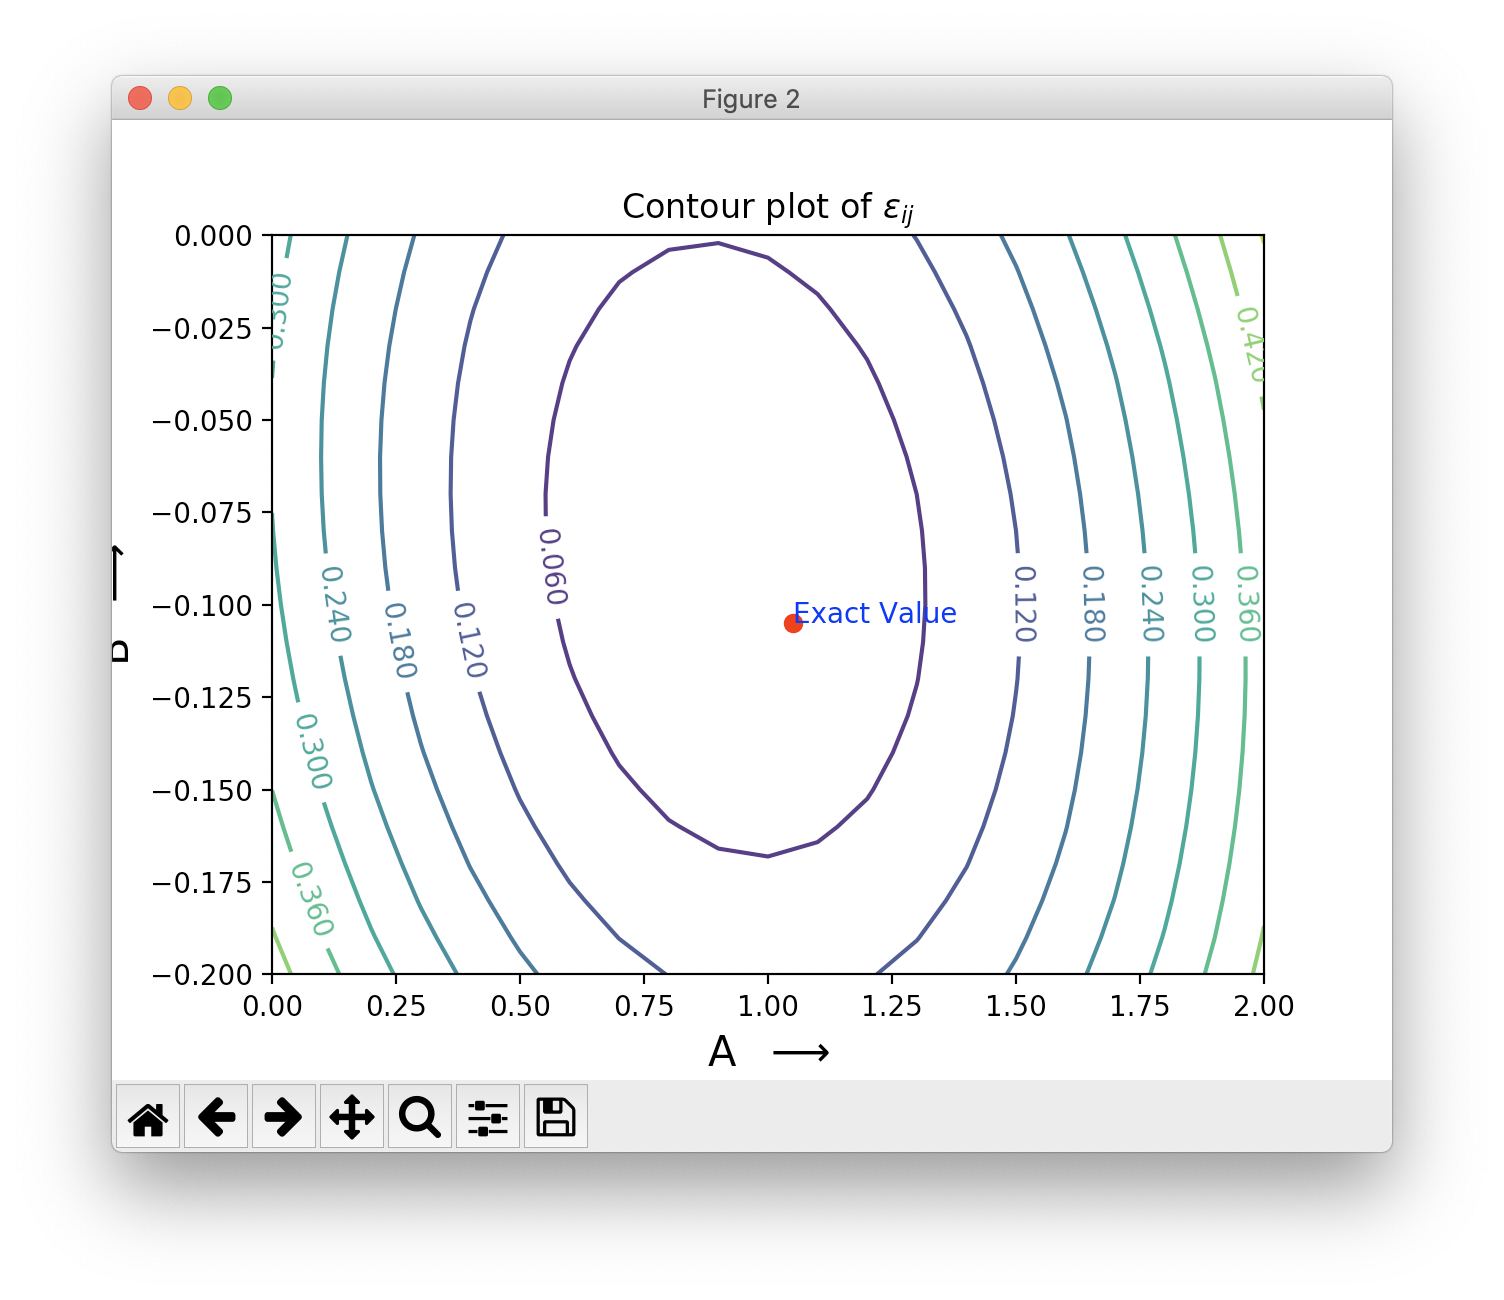
\includegraphics[scale=0.4]{scr3.png}}


\section{The Optimal Coefficients}
For calculation of optimal coefficients, I use the lstsq() function for the accurate prediction of coefficients
\begin{verbatim}
predict_coeff=array([zeros(k-1)]*(2))
for i in range(0,k-1):
	p,resid,rank,sig=lstsq(F,y_data[i])
	predict_coeff[0][i]=p[0]
	predict_coeff[1][i]=p[1]
\end{verbatim}
And the coefficients are stored in the arrays $predict\_coeff$ array.



% \chapter{Results}\label{chapt:results}

% \section{Plots:}


% % \section{Test 2} ... as needed

\chapter{Conclusions}
\section{On the Contour Plot of $\large\epsilon_{ij}$}
There is one minima for for every contour of $\epsilon$, 
and the co-ordinates of that minima are given by the output of lstsq() function.\par
So, on overall as there are nine readings, there are nine locations of minima of $\epsilon$, which corresponds to the nine pair of accurate coefficients, calculated from the lstsq() function.
\section{On the Linearity of Error (of $A's$ and $B's$) with the Standard Deviation}
The Error in the predicted coefficients with respect to the Actual coefficients is varying linearly with the standard deviation of the noise.
\pagebreak


\pagebreak

\end{document}

